% Options for packages loaded elsewhere
\PassOptionsToPackage{unicode}{hyperref}
\PassOptionsToPackage{hyphens}{url}
%
\documentclass[
]{article}
\usepackage{lmodern}
\usepackage{amssymb,amsmath}
\usepackage{ifxetex,ifluatex}
\ifnum 0\ifxetex 1\fi\ifluatex 1\fi=0 % if pdftex
  \usepackage[T1]{fontenc}
  \usepackage[utf8]{inputenc}
  \usepackage{textcomp} % provide euro and other symbols
\else % if luatex or xetex
  \usepackage{unicode-math}
  \defaultfontfeatures{Scale=MatchLowercase}
  \defaultfontfeatures[\rmfamily]{Ligatures=TeX,Scale=1}
\fi
% Use upquote if available, for straight quotes in verbatim environments
\IfFileExists{upquote.sty}{\usepackage{upquote}}{}
\IfFileExists{microtype.sty}{% use microtype if available
  \usepackage[]{microtype}
  \UseMicrotypeSet[protrusion]{basicmath} % disable protrusion for tt fonts
}{}
\makeatletter
\@ifundefined{KOMAClassName}{% if non-KOMA class
  \IfFileExists{parskip.sty}{%
    \usepackage{parskip}
  }{% else
    \setlength{\parindent}{0pt}
    \setlength{\parskip}{6pt plus 2pt minus 1pt}}
}{% if KOMA class
  \KOMAoptions{parskip=half}}
\makeatother
\usepackage{xcolor}
\IfFileExists{xurl.sty}{\usepackage{xurl}}{} % add URL line breaks if available
\IfFileExists{bookmark.sty}{\usepackage{bookmark}}{\usepackage{hyperref}}
\hypersetup{
  pdftitle={Intro to R for Decision Modeling},
  pdfauthor={SickKids and DARTH},
  hidelinks,
  pdfcreator={LaTeX via pandoc}}
\urlstyle{same} % disable monospaced font for URLs
\usepackage[margin=1in]{geometry}
\usepackage{color}
\usepackage{fancyvrb}
\newcommand{\VerbBar}{|}
\newcommand{\VERB}{\Verb[commandchars=\\\{\}]}
\DefineVerbatimEnvironment{Highlighting}{Verbatim}{commandchars=\\\{\}}
% Add ',fontsize=\small' for more characters per line
\usepackage{framed}
\definecolor{shadecolor}{RGB}{248,248,248}
\newenvironment{Shaded}{\begin{snugshade}}{\end{snugshade}}
\newcommand{\AlertTok}[1]{\textcolor[rgb]{0.94,0.16,0.16}{#1}}
\newcommand{\AnnotationTok}[1]{\textcolor[rgb]{0.56,0.35,0.01}{\textbf{\textit{#1}}}}
\newcommand{\AttributeTok}[1]{\textcolor[rgb]{0.77,0.63,0.00}{#1}}
\newcommand{\BaseNTok}[1]{\textcolor[rgb]{0.00,0.00,0.81}{#1}}
\newcommand{\BuiltInTok}[1]{#1}
\newcommand{\CharTok}[1]{\textcolor[rgb]{0.31,0.60,0.02}{#1}}
\newcommand{\CommentTok}[1]{\textcolor[rgb]{0.56,0.35,0.01}{\textit{#1}}}
\newcommand{\CommentVarTok}[1]{\textcolor[rgb]{0.56,0.35,0.01}{\textbf{\textit{#1}}}}
\newcommand{\ConstantTok}[1]{\textcolor[rgb]{0.00,0.00,0.00}{#1}}
\newcommand{\ControlFlowTok}[1]{\textcolor[rgb]{0.13,0.29,0.53}{\textbf{#1}}}
\newcommand{\DataTypeTok}[1]{\textcolor[rgb]{0.13,0.29,0.53}{#1}}
\newcommand{\DecValTok}[1]{\textcolor[rgb]{0.00,0.00,0.81}{#1}}
\newcommand{\DocumentationTok}[1]{\textcolor[rgb]{0.56,0.35,0.01}{\textbf{\textit{#1}}}}
\newcommand{\ErrorTok}[1]{\textcolor[rgb]{0.64,0.00,0.00}{\textbf{#1}}}
\newcommand{\ExtensionTok}[1]{#1}
\newcommand{\FloatTok}[1]{\textcolor[rgb]{0.00,0.00,0.81}{#1}}
\newcommand{\FunctionTok}[1]{\textcolor[rgb]{0.00,0.00,0.00}{#1}}
\newcommand{\ImportTok}[1]{#1}
\newcommand{\InformationTok}[1]{\textcolor[rgb]{0.56,0.35,0.01}{\textbf{\textit{#1}}}}
\newcommand{\KeywordTok}[1]{\textcolor[rgb]{0.13,0.29,0.53}{\textbf{#1}}}
\newcommand{\NormalTok}[1]{#1}
\newcommand{\OperatorTok}[1]{\textcolor[rgb]{0.81,0.36,0.00}{\textbf{#1}}}
\newcommand{\OtherTok}[1]{\textcolor[rgb]{0.56,0.35,0.01}{#1}}
\newcommand{\PreprocessorTok}[1]{\textcolor[rgb]{0.56,0.35,0.01}{\textit{#1}}}
\newcommand{\RegionMarkerTok}[1]{#1}
\newcommand{\SpecialCharTok}[1]{\textcolor[rgb]{0.00,0.00,0.00}{#1}}
\newcommand{\SpecialStringTok}[1]{\textcolor[rgb]{0.31,0.60,0.02}{#1}}
\newcommand{\StringTok}[1]{\textcolor[rgb]{0.31,0.60,0.02}{#1}}
\newcommand{\VariableTok}[1]{\textcolor[rgb]{0.00,0.00,0.00}{#1}}
\newcommand{\VerbatimStringTok}[1]{\textcolor[rgb]{0.31,0.60,0.02}{#1}}
\newcommand{\WarningTok}[1]{\textcolor[rgb]{0.56,0.35,0.01}{\textbf{\textit{#1}}}}
\usepackage{graphicx,grffile}
\makeatletter
\def\maxwidth{\ifdim\Gin@nat@width>\linewidth\linewidth\else\Gin@nat@width\fi}
\def\maxheight{\ifdim\Gin@nat@height>\textheight\textheight\else\Gin@nat@height\fi}
\makeatother
% Scale images if necessary, so that they will not overflow the page
% margins by default, and it is still possible to overwrite the defaults
% using explicit options in \includegraphics[width, height, ...]{}
\setkeys{Gin}{width=\maxwidth,height=\maxheight,keepaspectratio}
% Set default figure placement to htbp
\makeatletter
\def\fps@figure{htbp}
\makeatother
\setlength{\emergencystretch}{3em} % prevent overfull lines
\providecommand{\tightlist}{%
  \setlength{\itemsep}{0pt}\setlength{\parskip}{0pt}}
\setcounter{secnumdepth}{-\maxdimen} % remove section numbering

\title{Intro to R for Decision Modeling}
\usepackage{etoolbox}
\makeatletter
\providecommand{\subtitle}[1]{% add subtitle to \maketitle
  \apptocmd{\@title}{\par {\large #1 \par}}{}{}
}
\makeatother
\subtitle{Loops and Functions}
\author{SickKids and DARTH}
\date{11/2/2020}

\begin{document}
\maketitle

Change \texttt{eval} to \texttt{TRUE} if you want to knit this document.

This worksheet introduces the programming capabilities of \texttt{R}.
Programming in \texttt{R} can make it easier to perform repetitive
analyses such as sensitivity analysis and allow you to create your own
functions to perform specific data analysis for example. This session is
split into the following sections:

\begin{enumerate}
\def\labelenumi{\arabic{enumi}.}
\item
  Loops
\item
  Functions
\item
  The `apply' family
\end{enumerate}

Throughout the course, we will demonstrate code and leave some empty
\emph{code chunks} for you to fill in. We will also provide solutions
after the session.

Feel free to modify this document with your own comments and
clarifications.

\hypertarget{load-data-into-r}{%
\section{\texorpdfstring{0. Load data into
\texttt{R}}{0. Load data into R}}\label{load-data-into-r}}

Before we begin this session, we need to load our Framingham dataset
into \texttt{R}.

\begin{Shaded}
\begin{Highlighting}[]
\NormalTok{data <-}\StringTok{ }\KeywordTok{read.csv}\NormalTok{(}\StringTok{'framingham.csv'}\NormalTok{, }\DataTypeTok{header =} \OtherTok{TRUE}\NormalTok{)}
\end{Highlighting}
\end{Shaded}

We will modify a few important variables so that we can understand and
visualize the results better.

Nested \texttt{ifelse} statements should be read from `outside-in'. That
is, start with the most outer \texttt{ifelse} statement and work your
way in. For the purpose of working through these exercises, you do not
have to fully understand the code in the below code chunk.

\begin{Shaded}
\begin{Highlighting}[]
\KeywordTok{library}\NormalTok{(dplyr)}
\NormalTok{data1 <-}\StringTok{ }\NormalTok{data }\OperatorTok\StringTok{ }
\StringTok{             }\KeywordTok{mutate}\NormalTok{(}\DataTypeTok{SEX =} \KeywordTok{ifelse}\NormalTok{(}\OperatorTok{!}\KeywordTok{is.na}\NormalTok{(SEX), }
                                    \KeywordTok{ifelse}\NormalTok{(SEX }\OperatorTok{==}\StringTok{ }\DecValTok{1}\NormalTok{, }
                                           \StringTok{'male'}\NormalTok{, }\StringTok{'female'}\NormalTok{), }
                                 \OtherTok{NA}\NormalTok{)) }\OperatorTok
\StringTok{             }\KeywordTok{mutate}\NormalTok{(}\DataTypeTok{PREVSTRK =} \KeywordTok{ifelse}\NormalTok{(}\OperatorTok{!}\KeywordTok{is.na}\NormalTok{(PREVSTRK), }
                                         \KeywordTok{ifelse}\NormalTok{(PREVSTRK }\OperatorTok{==}\StringTok{ }\DecValTok{1}\NormalTok{, }
                                                \StringTok{'yes'}\NormalTok{, }\StringTok{'no'}\NormalTok{), }
                                      \OtherTok{NA}\NormalTok{)) }\OperatorTok
\StringTok{             }\KeywordTok{mutate}\NormalTok{(}\DataTypeTok{PREVMI =} \KeywordTok{ifelse}\NormalTok{(}\OperatorTok{!}\KeywordTok{is.na}\NormalTok{(PREVMI), }
                                       \KeywordTok{ifelse}\NormalTok{(PREVMI }\OperatorTok{==}\StringTok{ }\DecValTok{1}\NormalTok{, }
                                              \StringTok{'yes'}\NormalTok{, }\StringTok{'no'}\NormalTok{), }
                                    \OtherTok{NA}\NormalTok{)) }\OperatorTok\StringTok{ }
\StringTok{             }\KeywordTok{mutate}\NormalTok{(}\DataTypeTok{DIABETES =} \KeywordTok{ifelse}\NormalTok{(}\OperatorTok{!}\KeywordTok{is.na}\NormalTok{(DIABETES), }
                                         \KeywordTok{ifelse}\NormalTok{(DIABETES}\OperatorTok{==}\StringTok{ }\DecValTok{1}\NormalTok{, }
                                                \StringTok{'yes'}\NormalTok{, }\StringTok{'no'}\NormalTok{), }
                                      \OtherTok{NA}\NormalTok{)) }\OperatorTok
\StringTok{             }\KeywordTok{mutate}\NormalTok{(}\DataTypeTok{CURSMOKE =} \KeywordTok{ifelse}\NormalTok{(}\OperatorTok{!}\KeywordTok{is.na}\NormalTok{(CURSMOKE), }
                                         \KeywordTok{ifelse}\NormalTok{(CURSMOKE}\OperatorTok{==}\StringTok{ }\DecValTok{1}\NormalTok{, }
                                                \StringTok{'yes'}\NormalTok{, }\StringTok{'no'}\NormalTok{), }
                                      \OtherTok{NA}\NormalTok{)) }\OperatorTok
\StringTok{             }\KeywordTok{mutate}\NormalTok{(}\DataTypeTok{BPMEDS =} \KeywordTok{ifelse}\NormalTok{(}\OperatorTok{!}\KeywordTok{is.na}\NormalTok{(BPMEDS), }
                                       \KeywordTok{ifelse}\NormalTok{(BPMEDS}\OperatorTok{==}\StringTok{ }\DecValTok{1}\NormalTok{, }
                                              \StringTok{'yes'}\NormalTok{, }\StringTok{'no'}\NormalTok{), }
                                    \OtherTok{NA}\NormalTok{))}
\end{Highlighting}
\end{Shaded}

\hypertarget{loops}{%
\section{1. Loops}\label{loops}}

When programming in \texttt{R}, we often wish to execute an operation or
a combination of operations multiple times. If you are copying the same
code multiple times it may be easier to use loops to iterate. Both for
speed and readibility.

For creating loops we will be looking at \texttt{for}, \texttt{while},
\texttt{if} and \texttt{else} statements.

\hypertarget{for-loop}{%
\subsection{\texorpdfstring{\texttt{for}
loop}{for loop}}\label{for-loop}}

A \texttt{for} loop in R allows us to run a piece of code multiple times
and is structured as follows.

\begin{verbatim}
for(value in sequence){
 do something 
}
\end{verbatim}

The \texttt{value} is a character (we often use \texttt{i}), and the
\texttt{sequence} is a vector. For example, the following \texttt{for}
loop prints (outputs) the sqaure of each element in the vector
\texttt{Ages}:

\begin{Shaded}
\begin{Highlighting}[]
\NormalTok{Ages <-}\StringTok{ }\KeywordTok{c}\NormalTok{(}\DecValTok{5}\NormalTok{, }\DecValTok{10}\NormalTok{, }\DecValTok{12}\NormalTok{) }
\CommentTok{# For each age, square it}
\ControlFlowTok{for}\NormalTok{(i }\ControlFlowTok{in}\NormalTok{ Ages)\{}
  \KeywordTok{print}\NormalTok{(i }\OperatorTok{^}\StringTok{ }\DecValTok{2}\NormalTok{)}
\NormalTok{\}}
\end{Highlighting}
\end{Shaded}

\begin{verbatim}
## [1] 25
## [1] 100
## [1] 144
\end{verbatim}

Note that we used the \texttt{print()} function in the code above.
Typically \texttt{R} does not produce any output in the console or R
Markdown document when using a \texttt{for} loop. The \texttt{print()}
function is used to give output from the loop.

There are two key functions that are often used in conjunction with
\texttt{for} loops:

\begin{itemize}
\tightlist
\item
  The colon operator \texttt{:}, which creates a sequence from the
  number left of the \texttt{:} to the number right, increasing by 1 or
  -1, e.g.
\end{itemize}

\begin{Shaded}
\begin{Highlighting}[]
\DecValTok{1}\OperatorTok{:}\DecValTok{10}
\end{Highlighting}
\end{Shaded}

\begin{verbatim}
##  [1]  1  2  3  4  5  6  7  8  9 10
\end{verbatim}

\begin{Shaded}
\begin{Highlighting}[]
\DecValTok{4}\OperatorTok{:}\DecValTok{1} 
\end{Highlighting}
\end{Shaded}

\begin{verbatim}
## [1] 4 3 2 1
\end{verbatim}

\begin{itemize}
\tightlist
\item
  The \texttt{length()} function that returns the number of elements in
  a vector or list.
\end{itemize}

\begin{Shaded}
\begin{Highlighting}[]
\KeywordTok{length}\NormalTok{(Ages)}
\end{Highlighting}
\end{Shaded}

\begin{verbatim}
## [1] 3
\end{verbatim}

A common structure of a \texttt{for} loop uses the colon operator and
\texttt{length()} to perfom an operation for the \(i^{th}\) element in a
vector,

\begin{Shaded}
\begin{Highlighting}[]
\CommentTok{# For each age, square it}
\ControlFlowTok{for}\NormalTok{(i }\ControlFlowTok{in} \DecValTok{1}\OperatorTok{:}\KeywordTok{length}\NormalTok{(Ages))\{}
  \KeywordTok{print}\NormalTok{(Ages[i] }\OperatorTok{^}\StringTok{ }\DecValTok{2}\NormalTok{)}
\NormalTok{\}}
\end{Highlighting}
\end{Shaded}

\begin{verbatim}
## [1] 25
## [1] 100
## [1] 144
\end{verbatim}

The number of functions and mathematical operations that can be used
within a \texttt{for} loop is very large. So, \texttt{for} loops can get
very complex as you perform more complex operations.

\textbf{EXERCISE 1} Print the BMI multiplied by 2 for each of the first
ten subjects in the Framingham dataset.

\begin{Shaded}
\begin{Highlighting}[]
\CommentTok{# Your turn}
\ControlFlowTok{for}\NormalTok{ (i }\ControlFlowTok{in} \DecValTok{1}\OperatorTok{:}\DecValTok{10}\NormalTok{) \{}
   \KeywordTok{print}\NormalTok{(data1}\OperatorTok{$}\NormalTok{BMI[i] }\OperatorTok{*}\StringTok{ }\DecValTok{2}\NormalTok{)}
\NormalTok{\}}
\end{Highlighting}
\end{Shaded}

\begin{verbatim}
## [1] NA
## [1] 57
## [1] 49.22
## [1] 62.34
## [1] 44.04
## [1] 51.44
## [1] 58.22
## [1] 43.96
## [1] 53.24
## [1] 49.54
\end{verbatim}

Within the \texttt{for} loop it is also possible to assign values to
different elements in a vector. In the following code, we calculate the
mean age for males and females in Framingham dataset and save it to a
vector called \texttt{mean\_sex\_age}. \textbf{Notice that \emph{before}
saving the mean age for males and females in the vector
\texttt{mean\_sex\_age}, we have to create a vector called
\texttt{mean\_sex\_age} so \texttt{R} knows where to save the
calculations.} We usually create an empty vector of the right length to
store our results, e.g.,

\begin{Shaded}
\begin{Highlighting}[]
\CommentTok{# a vector containing the categories of the SEX variable for us to iterate over later}
\NormalTok{sex_index <-}\StringTok{ }\KeywordTok{c}\NormalTok{(}\StringTok{"male"}\NormalTok{, }\StringTok{"female"}\NormalTok{)}
\CommentTok{# create an empty vector store the result of our for loop}
\NormalTok{mean_sex_age <-}\StringTok{ }\KeywordTok{vector}\NormalTok{(}\DataTypeTok{length =} \KeywordTok{length}\NormalTok{(sex_index))}
\CommentTok{# the names() function gives names to the elements in a vector}
\KeywordTok{names}\NormalTok{(mean_sex_age) <-}\StringTok{ }\NormalTok{sex_index}

\CommentTok{# set up and run the for loop}
\ControlFlowTok{for}\NormalTok{ (i }\ControlFlowTok{in} \DecValTok{1}\OperatorTok{:}\KeywordTok{length}\NormalTok{(sex_index)) \{}
\NormalTok{  mean_sex_age[i] <-}\StringTok{ }\KeywordTok{mean}\NormalTok{(}
\NormalTok{  data1}\OperatorTok{$}\NormalTok{AGE[data1}\OperatorTok{$}\NormalTok{SEX }\OperatorTok{==}\StringTok{ }\NormalTok{sex_index[i]]}
\NormalTok{  )}
\NormalTok{\}}

\CommentTok{# display the results}
\NormalTok{mean_sex_age}
\end{Highlighting}
\end{Shaded}

\begin{verbatim}
##     male   female 
## 60.34895 60.86940
\end{verbatim}

\hypertarget{if-and-else-statement}{%
\subsection{\texorpdfstring{\texttt{if} and \texttt{else}
statement}{if and else statement}}\label{if-and-else-statement}}

An \texttt{if} statement is used to perform an action when a specific
statement is true. The syntax for an \texttt{if} statement is:

\begin{verbatim}
if (expression) {
statement
}
\end{verbatim}

If the \texttt{expression} is \texttt{TRUE}, the code in the
\texttt{statement} is run. If the \texttt{expression} is \texttt{FALSE},
nothing happens.

\textbf{EXERCISE 2} The following code prints ``negative number'' if
\texttt{x} is negative, test this statement with different values for
\texttt{x}.

\begin{Shaded}
\begin{Highlighting}[]
\CommentTok{# Your turn}
\NormalTok{x <-}\StringTok{ }\DecValTok{5}
\ControlFlowTok{if}\NormalTok{ (x }\OperatorTok{<}\StringTok{ }\DecValTok{0}\NormalTok{) \{}
    \KeywordTok{print}\NormalTok{(}\StringTok{"negative number"}\NormalTok{)}
\NormalTok{\}}
\end{Highlighting}
\end{Shaded}

It is possible to follow \texttt{if} by \texttt{else} to create a
\texttt{if...else} statement. The syntax is:

\begin{verbatim}
if (expression) {
statement1
} else {
statement2
}
\end{verbatim}

The \texttt{else} component is optional and is only evaluated if the
expression is FALSE.

\textbf{ExERCISE 3} Create an \texttt{if...else} statement that prints
``negative number'' if \texttt{x} is less than 0 and ``not a negative
number'' if \texttt{x} is not. Test your statement with different values
for \texttt{x}.

\begin{Shaded}
\begin{Highlighting}[]
\CommentTok{# Your turn}
\NormalTok{x <-}\StringTok{ }\DecValTok{-10}
\ControlFlowTok{if}\NormalTok{ (x }\OperatorTok{<}\StringTok{ }\DecValTok{0}\NormalTok{) \{}
   \KeywordTok{print}\NormalTok{(}\StringTok{"negative number"}\NormalTok{)}
\NormalTok{\} }\ControlFlowTok{else}\NormalTok{ \{}
  \KeywordTok{print}\NormalTok{(}\StringTok{"not a negative number"}\NormalTok{)}
\NormalTok{\}}
\end{Highlighting}
\end{Shaded}

\begin{verbatim}
## [1] "negative number"
\end{verbatim}

You can also have another \texttt{if} with an expression followed by
\texttt{else} as follows:

\begin{verbatim}
if (expression 1) {
statement1
} else if (expression 2) {
statement2
}
\end{verbatim}

\textbf{ExERCISE 4} Create an \texttt{if...else} statement that prints
``negative number'' if \texttt{x} is less than 0 and ``positive number''
if \texttt{x} is greater than 0. Test your statement with different
values for \texttt{x}.

\begin{Shaded}
\begin{Highlighting}[]
\CommentTok{# Your turn}
\NormalTok{x <-}\StringTok{ }\DecValTok{10}
\ControlFlowTok{if}\NormalTok{ (x }\OperatorTok{<}\StringTok{ }\DecValTok{0}\NormalTok{) \{}
   \KeywordTok{print}\NormalTok{(}\StringTok{"negative number"}\NormalTok{)}
\NormalTok{\} }\ControlFlowTok{else} \ControlFlowTok{if}\NormalTok{ (x }\OperatorTok{>}\StringTok{ }\DecValTok{0}\NormalTok{) \{}
  \KeywordTok{print}\NormalTok{(}\StringTok{"positive number"}\NormalTok{)}
\NormalTok{\}}
\end{Highlighting}
\end{Shaded}

\begin{verbatim}
## [1] "positive number"
\end{verbatim}

We can combine \texttt{if...else} statements with \texttt{for} loops to
create powerful tools for data analysis and data manipulation. For
example,

\begin{Shaded}
\begin{Highlighting}[]
\NormalTok{y <-}\StringTok{ }\KeywordTok{c}\NormalTok{(}\DecValTok{1}\NormalTok{, }\DecValTok{3}\NormalTok{, }\DecValTok{10}\NormalTok{, }\DecValTok{-1}\NormalTok{, }\DecValTok{122}\NormalTok{, }\DecValTok{-9}\NormalTok{, }\DecValTok{-200}\NormalTok{)}
\ControlFlowTok{for}\NormalTok{ (i }\ControlFlowTok{in} \DecValTok{1}\OperatorTok{:}\KeywordTok{length}\NormalTok{(y)) \{}
  \ControlFlowTok{if}\NormalTok{ (y[i] }\OperatorTok{>}\StringTok{ }\DecValTok{0}\NormalTok{) \{}
  \KeywordTok{print}\NormalTok{(}\StringTok{'positive'}\NormalTok{)}
\NormalTok{  \} }
  \ControlFlowTok{else} \ControlFlowTok{if}\NormalTok{ (y[i] }\OperatorTok{<}\StringTok{ }\DecValTok{0}\NormalTok{) \{}
  \KeywordTok{print}\NormalTok{(}\StringTok{'negative'}\NormalTok{)}
\NormalTok{  \}}
\NormalTok{\}}
\end{Highlighting}
\end{Shaded}

\begin{verbatim}
## [1] "positive"
## [1] "positive"
## [1] "positive"
## [1] "negative"
## [1] "positive"
## [1] "negative"
## [1] "negative"
\end{verbatim}

The code above loops through the vector \texttt{y} and prints `positive'
if the \texttt{i}-th element is greater than 0 and `negative' if it is
less than 0.

\textbf{EXERCISE 5} Store the subject id (\texttt{RANDID}) of all
subjects over 70 years old in a vector and display it using
\texttt{for}, \texttt{if} and \texttt{else}. Check your answer by using
\texttt{filter()} and \texttt{select()} from the \texttt{dplyr} package.

\begin{Shaded}
\begin{Highlighting}[]
\CommentTok{# Your turn}
\NormalTok{age_}\DecValTok{70}\NormalTok{_index <-}\StringTok{ }\KeywordTok{vector}\NormalTok{(}\DataTypeTok{length =} \KeywordTok{length}\NormalTok{(data1}\OperatorTok{$}\NormalTok{AGE))}
\ControlFlowTok{for}\NormalTok{ (i }\ControlFlowTok{in} \DecValTok{1}\OperatorTok{:}\KeywordTok{nrow}\NormalTok{(data1)) \{}
  \ControlFlowTok{if}\NormalTok{ (data1}\OperatorTok{$}\NormalTok{AGE[i] }\OperatorTok{==}\StringTok{ }\DecValTok{70}\NormalTok{) \{}
\NormalTok{     age_}\DecValTok{70}\NormalTok{_index[i] <-}\StringTok{ }\DecValTok{1} 
\NormalTok{  \}}
\NormalTok{\}}
\NormalTok{age_}\DecValTok{70}\NormalTok{ <-}\StringTok{ }\NormalTok{data}\OperatorTok{$}\NormalTok{RANDID[age_}\DecValTok{70}\NormalTok{_index }\OperatorTok{==}\StringTok{ }\DecValTok{1}\NormalTok{]}
\NormalTok{age_}\DecValTok{70}\NormalTok{[}\DecValTok{1}\OperatorTok{:}\DecValTok{6}\NormalTok{]}
\end{Highlighting}
\end{Shaded}

\begin{verbatim}
## [1] 390449 491826 571377 610146 814971 968768
\end{verbatim}

\begin{Shaded}
\begin{Highlighting}[]
\CommentTok{# check answer}
\NormalTok{data1 }\OperatorTok\StringTok{ }
\StringTok{     }\KeywordTok{filter}\NormalTok{(AGE }\OperatorTok{==}\StringTok{ }\DecValTok{70}\NormalTok{) }\OperatorTok
\StringTok{     }\KeywordTok{select}\NormalTok{(RANDID) }\OperatorTok
\StringTok{     }\KeywordTok{head}\NormalTok{()}
\end{Highlighting}
\end{Shaded}

\begin{verbatim}
##   RANDID
## 1 390449
## 2 491826
## 3 571377
## 4 610146
## 5 814971
## 6 968768
\end{verbatim}

\hypertarget{functions}{%
\section{2. Functions}\label{functions}}

Almost all operations in \texttt{R} are achieved using \emph{functions}.
The general syntax for \emph{functions} is
\texttt{function\_name(arguments)} We have seen many of them until now
(e.g.~\texttt{mean()}, \texttt{max()}, \texttt{quantile()}). These are
pre-specified (built-in) functions in \texttt{R}.

In some settings, pre-specified functions in \texttt{R} are not
sufficient for the analysis we would like to perform. In such cases, it
is good practice to define your own functions to perform analyses. This
can help you reproduce your analysis at a later date and repeat the same
analysis on another dataset.

The generally syntax for writing your own function is as follows:

\begin{verbatim}
function_name <- function(arguments) {
   ...
   return(output)
}
\end{verbatim}

The function can have a large number of \texttt{arguments}, or function
inputs, separated by commas. The \texttt{output} from a function can
have multiple elements that should be returned as a list.

\begin{verbatim}
function_name <- function(argument1, argument2, argument3) {
   ...
   return(list(output1, output2, output3)
}
\end{verbatim}

Once a function has been defined using the code above, it can be used as
a standard function in \texttt{R}.

For example, the following function calculates the mean of a vector:

\begin{Shaded}
\begin{Highlighting}[]
\CommentTok{# Write our own function to calculate the mean}
\NormalTok{mean_own <-}\StringTok{ }\ControlFlowTok{function}\NormalTok{(data)\{}
\NormalTok{   mean_calc <-}\StringTok{ }\KeywordTok{sum}\NormalTok{(data) }\OperatorTok{/}\StringTok{ }\KeywordTok{length}\NormalTok{(data)}
   \KeywordTok{return}\NormalTok{(mean_calc)}
\NormalTok{\}}
\KeywordTok{mean_own}\NormalTok{(}\DecValTok{1}\OperatorTok{:}\DecValTok{10}\NormalTok{)}
\end{Highlighting}
\end{Shaded}

\begin{verbatim}
## [1] 5.5
\end{verbatim}

\begin{Shaded}
\begin{Highlighting}[]
\CommentTok{# test}
\KeywordTok{mean}\NormalTok{(}\DecValTok{1}\OperatorTok{:}\DecValTok{10}\NormalTok{)}
\end{Highlighting}
\end{Shaded}

\begin{verbatim}
## [1] 5.5
\end{verbatim}

\textbf{EXERCISE 6} Write a function that converts Fahrenheit to
Celsius. The formula is (F-12) * 5 / 9. Test your function on 100
degrees Fahrenheit.

\begin{Shaded}
\begin{Highlighting}[]
\CommentTok{# Your turn}
\NormalTok{F_to_C <-}\StringTok{ }\ControlFlowTok{function}\NormalTok{(temperature_F) \{}
\NormalTok{   temperature_C <-}\StringTok{ }\NormalTok{(temperature_F }\OperatorTok{-}\StringTok{ }\DecValTok{32}\NormalTok{) }\OperatorTok{*}\StringTok{ }\DecValTok{5} \OperatorTok{/}\StringTok{ }\DecValTok{9}
   \KeywordTok{return}\NormalTok{(temperature_C)}
\NormalTok{\}}
\CommentTok{# test }
\KeywordTok{F_to_C}\NormalTok{(}\DecValTok{100}\NormalTok{)}
\end{Highlighting}
\end{Shaded}

\begin{verbatim}
## [1] 37.77778
\end{verbatim}

\textbf{EXERCISE 7} Write a function that calculates the square root of
the sum of the squares of two numbers. Test your function on 3 and 4.
The answer should be 5.

\begin{Shaded}
\begin{Highlighting}[]
\CommentTok{# Your turn}
\NormalTok{root_sum_of_squares <-}\StringTok{ }\ControlFlowTok{function}\NormalTok{ (x, y) \{}
\NormalTok{   root_sum_squares <-}\StringTok{ }\KeywordTok{sqrt}\NormalTok{(x }\OperatorTok{^}\StringTok{ }\DecValTok{2} \OperatorTok{+}\StringTok{ }\NormalTok{y }\OperatorTok{^}\StringTok{ }\DecValTok{2}\NormalTok{)}
   \KeywordTok{return}\NormalTok{(root_sum_squares)}
\NormalTok{\}}

\CommentTok{# test}
\KeywordTok{root_sum_of_squares}\NormalTok{(}\DecValTok{3}\NormalTok{,}\DecValTok{4}\NormalTok{)}
\end{Highlighting}
\end{Shaded}

\begin{verbatim}
## [1] 5
\end{verbatim}

\begin{Shaded}
\begin{Highlighting}[]
\KeywordTok{sqrt}\NormalTok{(}\DecValTok{3} \OperatorTok{^}\StringTok{ }\DecValTok{2} \OperatorTok{+}\StringTok{ }\DecValTok{4} \OperatorTok{^}\StringTok{ }\DecValTok{2}\NormalTok{)}
\end{Highlighting}
\end{Shaded}

\begin{verbatim}
## [1] 5
\end{verbatim}

You can write any number of operations between the left curly bracket
\texttt{\{} and the right curly bracket \texttt{\}}. All these
operations will be included in the function so you can perform the same
operations on different datasets.

Functions can be combined with loops to perform complex operations but
as these functions and loops become more complex, it is good practice to
insert comments within your functions.

Below we create our own summary function that calculates the mean,
standard deviation, minima and maxima of a vector. We use it on the age
variable in the framingham dataset.

\begin{Shaded}
\begin{Highlighting}[]
\CommentTok{# Write a function to summarize data}
\NormalTok{summary_own <-}\StringTok{ }\ControlFlowTok{function}\NormalTok{(data) \{}
  \CommentTok{# summary statistics}
\NormalTok{   mean_calc <-}\StringTok{ }\KeywordTok{sum}\NormalTok{(data) }\OperatorTok{/}\StringTok{ }\KeywordTok{length}\NormalTok{(data)}
\NormalTok{   sd_calc <-}\StringTok{ }\KeywordTok{sd}\NormalTok{(data)}
\NormalTok{   min_calc <-}\StringTok{ }\KeywordTok{min}\NormalTok{(data)}
\NormalTok{   max_calc <-}\KeywordTok{max}\NormalTok{(data)}
   \CommentTok{# name the summary statistics}
\NormalTok{   summaries <-}\StringTok{ }\KeywordTok{c}\NormalTok{(mean_calc,sd_calc,min_calc,max_calc)}
   \KeywordTok{names}\NormalTok{(summaries) <-}\StringTok{ }\KeywordTok{c}\NormalTok{(}\StringTok{'mean'}\NormalTok{, }\StringTok{'sd'}\NormalTok{, }\StringTok{'min'}\NormalTok{, }\StringTok{'max'}\NormalTok{)}
   \KeywordTok{return}\NormalTok{(summaries)}
\NormalTok{\}}

\CommentTok{# use it on AGE and store the ouptut in a object}
\NormalTok{age_summary <-}\StringTok{ }\KeywordTok{summary_own}\NormalTok{(data}\OperatorTok{$}\NormalTok{AGE)}
\CommentTok{# print the results}
\NormalTok{age_summary}
\end{Highlighting}
\end{Shaded}

\begin{verbatim}
##      mean        sd       min       max 
## 60.648177  8.296766 44.000000 81.000000
\end{verbatim}

\textbf{EXERCISE 8} Write a function that tests whether the mean
systolic blood pressure (\texttt{SYSBP}) is different for those who have
prevalent stroke (\texttt{PREVSTRK}) and those who do not and produces a
box plot of systolic blood pressure stratified by prevalent stroke
status with an appropriate title and labels. The function takes our
framingham dataset as the only argument.

\begin{Shaded}
\begin{Highlighting}[]
\CommentTok{# Your turn}
\NormalTok{test_sysbp <-}\StringTok{ }\ControlFlowTok{function}\NormalTok{ (data) \{}
\NormalTok{                no_PREVSTRK_SYSBP <-}\StringTok{ }\NormalTok{data}\OperatorTok{$}\NormalTok{SYSBP[data}\OperatorTok{$}\NormalTok{PREVSTRK }
                                                \OperatorTok{==}\StringTok{ 'no'}\NormalTok{]}
\NormalTok{                PREVSTRK_SYSBP <-}\StringTok{ }\NormalTok{data}\OperatorTok{$}\NormalTok{SYSBP[data}\OperatorTok{$}\NormalTok{PREVSTRK }
                                             \OperatorTok{==}\StringTok{ 'yes'}\NormalTok{]}
                \KeywordTok{boxplot}\NormalTok{(SYSBP }\OperatorTok{~}\StringTok{ }\NormalTok{PREVSTRK, }\DataTypeTok{data =}\NormalTok{ data, }
                        \DataTypeTok{main =} \StringTok{'Systolic blood pressure by }
\StringTok{                                prevalent stroke status'}\NormalTok{, }
                        \DataTypeTok{xlab =} \StringTok{'prevalent stroke'}\NormalTok{,}
                        \DataTypeTok{ylab =} \StringTok{'systolic blood pressure'}\NormalTok{)}
                \KeywordTok{return}\NormalTok{(}\KeywordTok{t.test}\NormalTok{(no_PREVSTRK_SYSBP, PREVSTRK_SYSBP))}
\NormalTok{\}}
\KeywordTok{test_sysbp}\NormalTok{(data1)}
\end{Highlighting}
\end{Shaded}

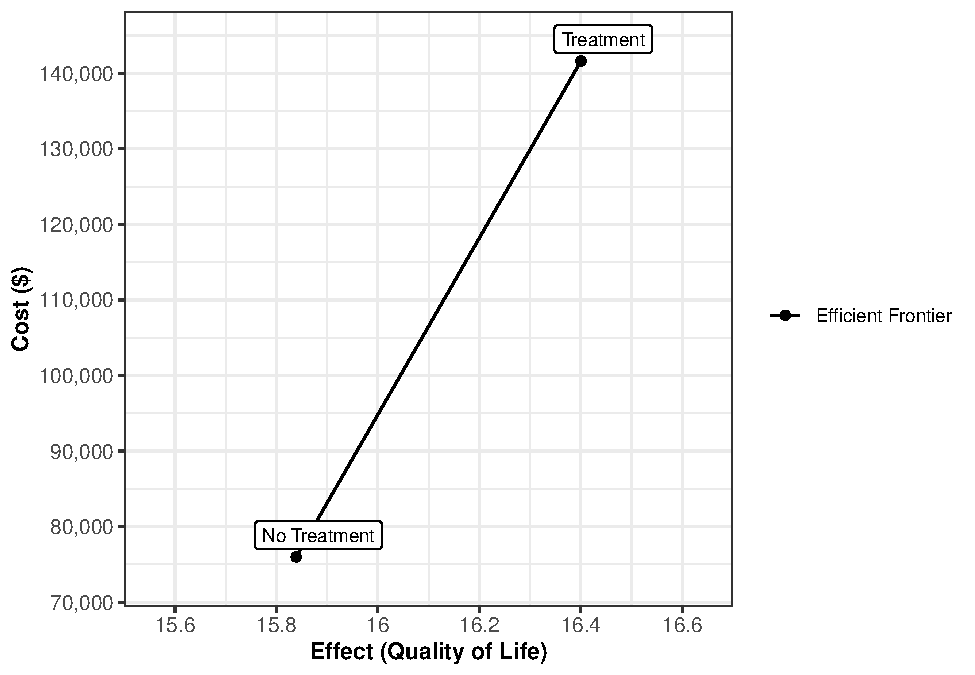
\includegraphics{05_loops_and_functions_solutions_files/figure-latex/unnamed-chunk-18-1.pdf}

\begin{verbatim}
## 
##  Welch Two Sample t-test
## 
## data:  no_PREVSTRK_SYSBP and PREVSTRK_SYSBP
## t = -6.9149, df = 71.276, p-value = 1.654e-09
## alternative hypothesis: true difference in means is not equal to 0
## 95 percent confidence interval:
##  -23.56921 -13.01937
## sample estimates:
## mean of x mean of y 
##  139.8289  158.1232
\end{verbatim}

\hypertarget{the-apply-family}{%
\section{3. The `apply' family}\label{the-apply-family}}

\texttt{R} can be quite slow if you use a \texttt{for} loop to
repeatedly use the same function across different elements of a dataset,
or multiple datasets. \texttt{R} is much faster when we use a family of
functions called the \texttt{apply} function. These functions, such as
\texttt{sapply()} function or \texttt{lapply()} are used to repeatedly
\emph{apply} the same function to a dataset or a list of different
datasets.

\texttt{sapply()} and \texttt{lapply()} take a list as its 1st argument
and a function as its 2nd argument. It calls the function on each item
in the list. The first \emph{code chunk} demonstrates the \texttt{for}
loop that we could use to calculate the summary statistics using our
function for the age of both males and females.

\begin{Shaded}
\begin{Highlighting}[]
\NormalTok{sex_index <-}\StringTok{ }\KeywordTok{c}\NormalTok{(}\StringTok{"male"}\NormalTok{, }\StringTok{"female"}\NormalTok{)}
\CommentTok{# create an dummy matrix to store the summary statistics}
\NormalTok{summary_sex_age <-}\StringTok{ }\KeywordTok{matrix}\NormalTok{(}\DecValTok{0}\NormalTok{, }\DataTypeTok{nrow =} \DecValTok{4}\NormalTok{, }\DataTypeTok{ncol =} \KeywordTok{length}\NormalTok{(sex_index))}
\CommentTok{# name the columns of the matrix}
\KeywordTok{colnames}\NormalTok{(summary_sex_age) <-}\StringTok{ }\NormalTok{sex_index}
\CommentTok{# use for loop to calculate the statistics }
\ControlFlowTok{for}\NormalTok{ (i }\ControlFlowTok{in} \DecValTok{1}\OperatorTok{:}\KeywordTok{length}\NormalTok{(sex_index)) \{}
\NormalTok{  summary_sex_age[,i] <-}\StringTok{ }\KeywordTok{summary_own}\NormalTok{(}
\NormalTok{  data1}\OperatorTok{$}\NormalTok{AGE[data1}\OperatorTok{$}\NormalTok{SEX }\OperatorTok{==}\StringTok{ }\NormalTok{sex_index[i]]}
\NormalTok{  )}
\NormalTok{\}}
\CommentTok{# display the results}
\NormalTok{summary_sex_age}
\end{Highlighting}
\end{Shaded}

\begin{verbatim}
##           male    female
## [1,] 60.348955 60.869403
## [2,]  8.191481  8.369054
## [3,] 45.000000 44.000000
## [4,] 80.000000 81.000000
\end{verbatim}

The \texttt{sapply()} function can be used to avoid the \texttt{for}
loop:

\begin{Shaded}
\begin{Highlighting}[]
\CommentTok{# create a list containing the ages for males and females separately}
\NormalTok{age_list <-}\StringTok{ }\KeywordTok{list}\NormalTok{(data1}\OperatorTok{$}\NormalTok{AGE[data1}\OperatorTok{$}\NormalTok{SEX }\OperatorTok{==}\StringTok{ }\NormalTok{sex_index[}\DecValTok{1}\NormalTok{]],}
\NormalTok{                 data1}\OperatorTok{$}\NormalTok{AGE[data1}\OperatorTok{$}\NormalTok{SEX }\OperatorTok{==}\StringTok{ }\NormalTok{sex_index[}\DecValTok{2}\NormalTok{]])}
\CommentTok{# use sapply to calculate the summary statistics}
\NormalTok{summary_sex_age1 <-}\StringTok{ }\KeywordTok{sapply}\NormalTok{(age_list, summary_own)}
\CommentTok{# name the rows}
\KeywordTok{colnames}\NormalTok{(summary_sex_age1) <-}\StringTok{ }\NormalTok{sex_index}
\CommentTok{# display the results}
\NormalTok{summary_sex_age1}
\end{Highlighting}
\end{Shaded}

\begin{verbatim}
##           male    female
## mean 60.348955 60.869403
## sd    8.191481  8.369054
## min  45.000000 44.000000
## max  80.000000 81.000000
\end{verbatim}

We can also use the \texttt{apply()} to apply a function to the rows or
columns (or both) of a data frame. While \texttt{lapply()} requires a
list input and returns a list instead of a vector as we saw for
\texttt{sapply()}.

\textbf{EXERCISE 9} We have created a list of temperatures in
Fahrenheit. Use the \texttt{sapply()} or \texttt{lapply()} functions to
convert them to Celsius.

\begin{Shaded}
\begin{Highlighting}[]
\CommentTok{# Your turn}
\NormalTok{F_temperatures <-}\StringTok{ }\KeywordTok{list}\NormalTok{(}\DecValTok{50}\NormalTok{, }\DecValTok{62}\NormalTok{, }\DecValTok{81}\NormalTok{, }\DecValTok{102}\NormalTok{, }\DecValTok{157}\NormalTok{) }
\KeywordTok{lapply}\NormalTok{(F_temperatures, F_to_C)}
\end{Highlighting}
\end{Shaded}

\begin{verbatim}
## [[1]]
## [1] 10
## 
## [[2]]
## [1] 16.66667
## 
## [[3]]
## [1] 27.22222
## 
## [[4]]
## [1] 38.88889
## 
## [[5]]
## [1] 69.44444
\end{verbatim}

\begin{Shaded}
\begin{Highlighting}[]
\KeywordTok{sapply}\NormalTok{(F_temperatures, F_to_C)}
\end{Highlighting}
\end{Shaded}

\begin{verbatim}
## [1] 10.00000 16.66667 27.22222 38.88889 69.44444
\end{verbatim}

\end{document}
